\chapter{Evaluation}
\label{chap:evaluation}

Five experiments were performed to validate the functionality of the tags.
The first is non specific and ment to test the setup in a stable environment.
Experiments two to four are intended to test the detection of unwanted circumstances.
Experiment five is tests the system in a real-world environment.
The experiment results were stored on the phone and then exported using email.
The analysis of the data and creation of graphs was then performed using a Jupiter Notebook, using Pandas and Pyplot for datamanagment and the creation of graphs.\\
For all experiments the query-frequency was set to 330s.
The measurements queries are spread across this timeframe.
Each experiment lasted between 40 minutes and one hour.
All eperiments were performed two to three times.
In each section only the data-set from the first experiment run is presented fully.
The other experiments will be mentioned only, if they have differing data or to confrim an unexpected datapoint.

The tags used were programmed as described in Chapter \ref{c:implementation}.
The same four tags were used for all experiments.
They will be refered to as Tag-1, Tag-2, Tag-3 and Tag-4.





\section{Experiment 1: Static}
\label{ss:exp_1}
The four tags where placed on the corners of a 80 cm by 50 cm rectangle on a wooden table.
Figure \ref{f:exp1_schematic} shows a schematic view of the setup.
Each tag was turned on sequentially and given enough time to establish the network.
The phone then was connected to Tag-4.
The parameters in the app were left unchanged.
The default parameters are large enough, that no measurement should be able to trigger a warning.
Orientational reading was used for the output of the gyroscope.
The setup was then left untouched for 35 min.
The goal of this experiment was, to gauge by how much the measurements can vary in a static environment.

\begin{figure}[ht!]
	\centering
	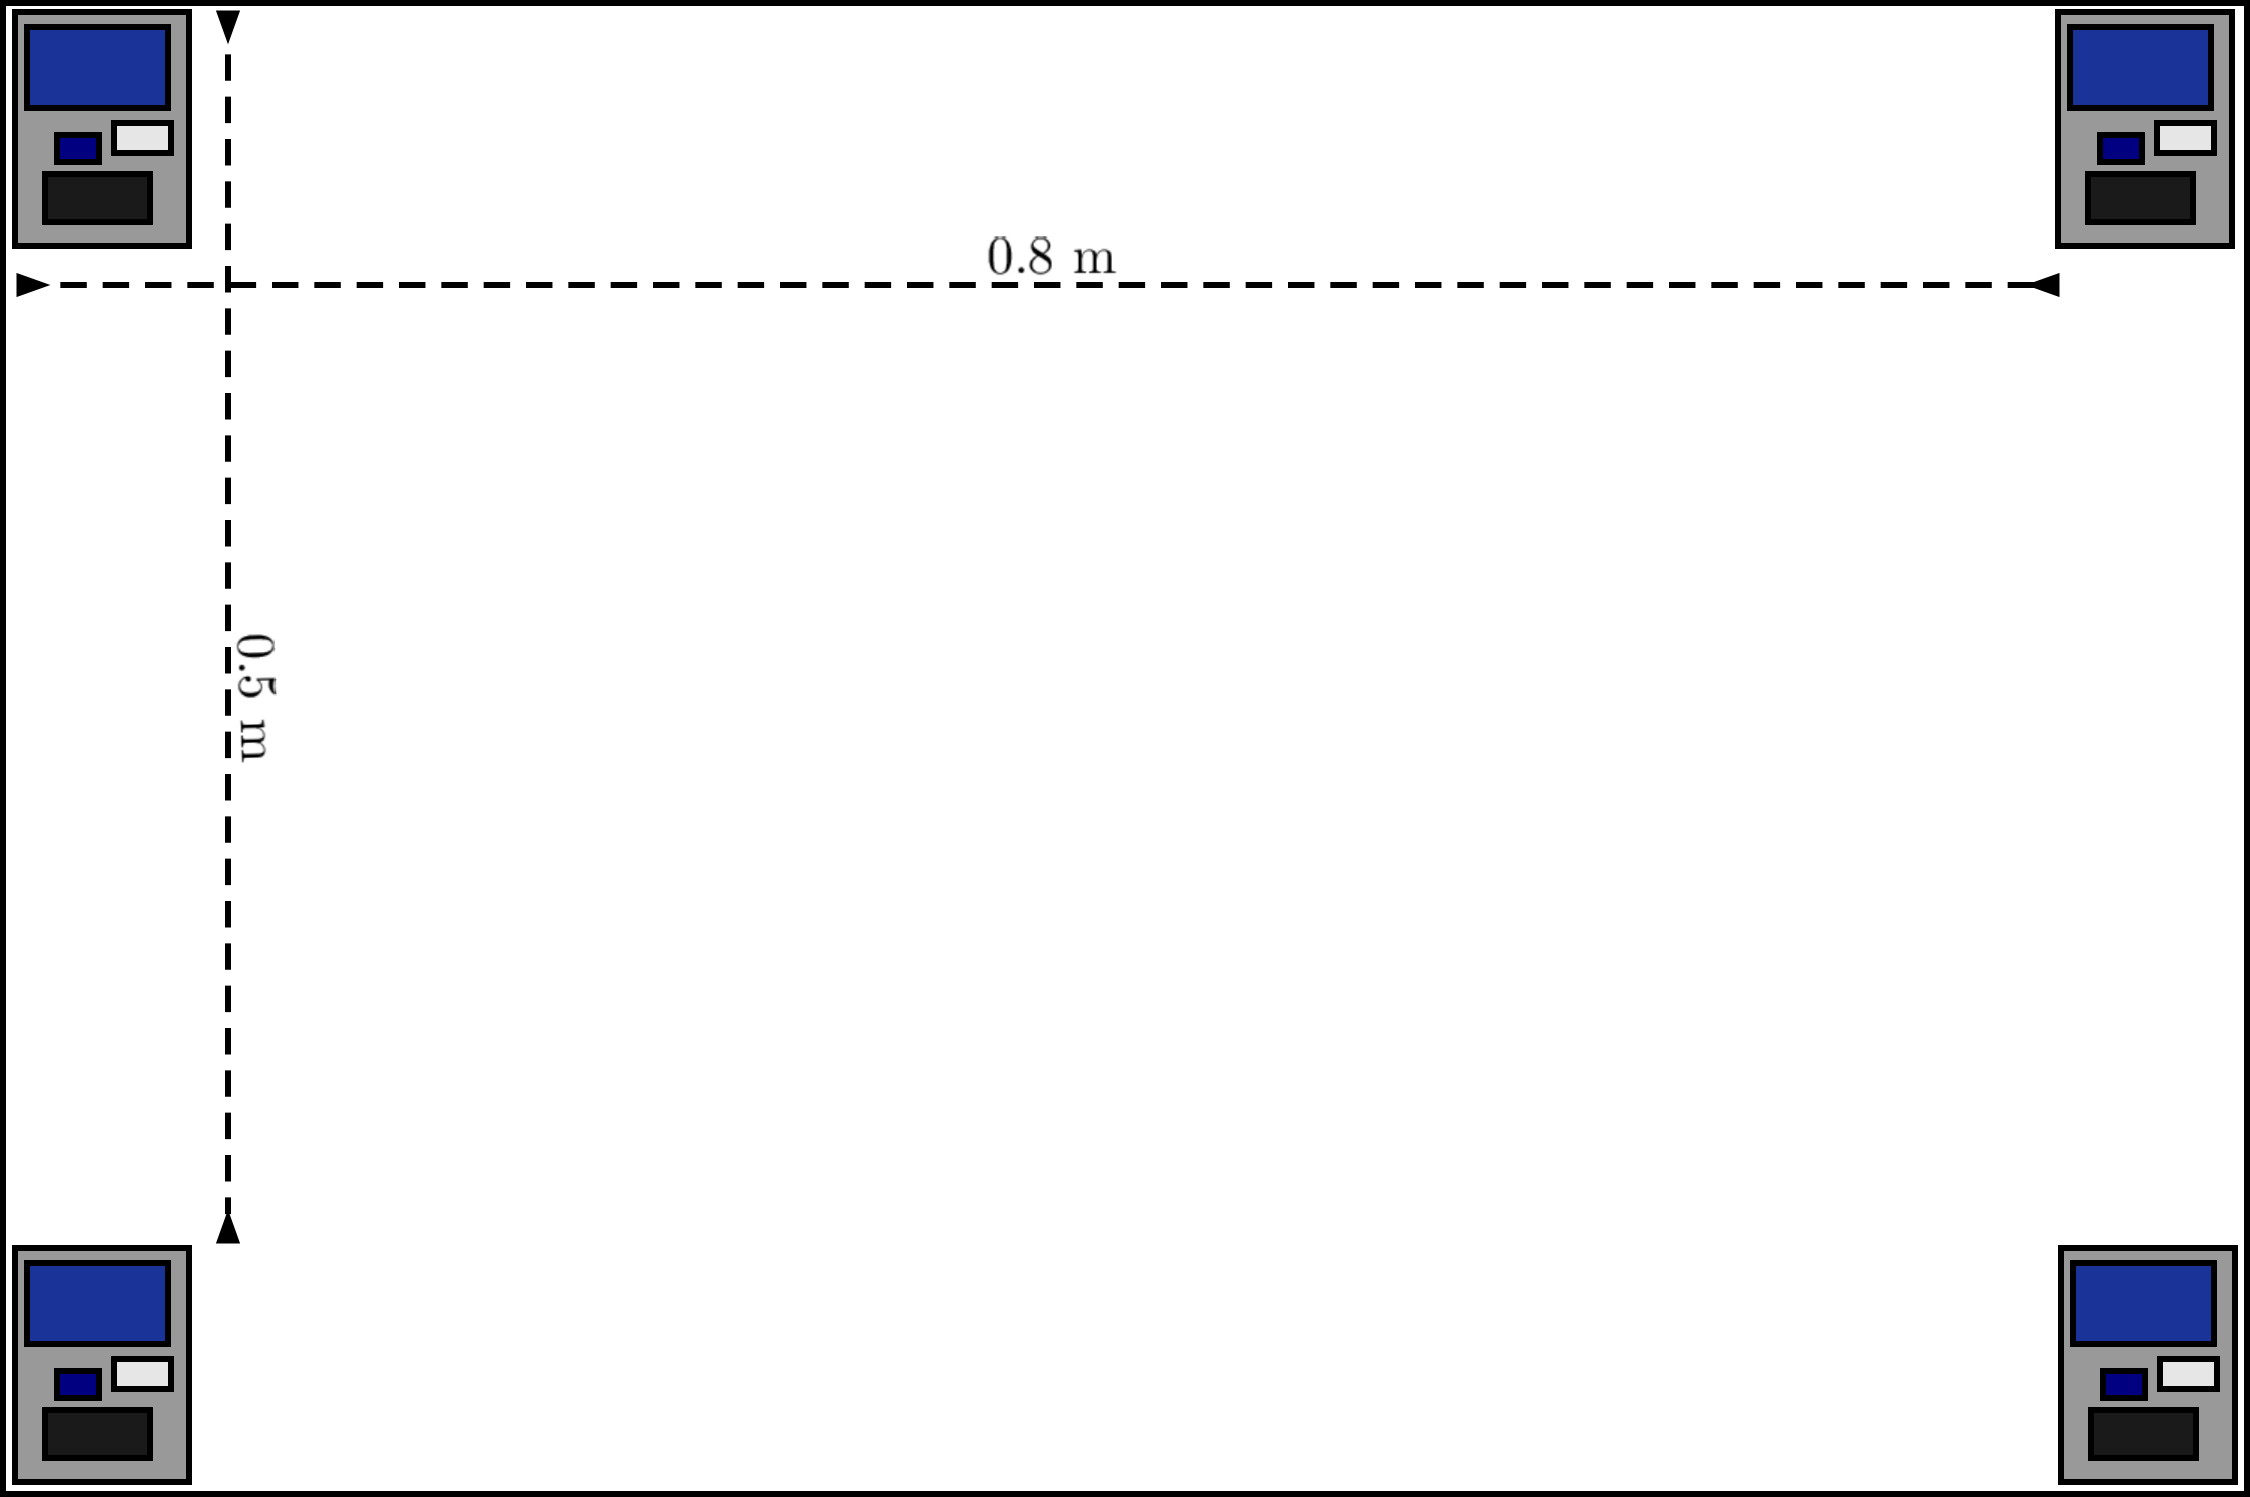
\includegraphics[width=300px]{graphics/schematics/experiment_1.png}
	\caption{Schema of the setup of experiment 1.}
	\label{f:exp1_schematic}
\end{figure}


\subsection{Results}
\label{ss:exp_1_result}
In eperiment one, all measurements are expected to be unchanging.
Table \ref{t:exp1_means} shows the mean values for temperature, humidity and angle during the experiment by tag.
Figures \ref{f:exp1_graphs_temp}, \ref{f:exp1_graphs_hum}, \ref{f:exp1_graphs_gyro}, \ref{f:exp1_graphs_dist} shows the change of these values over time.

\begin{table}[ht]
\centering
\caption{Mean and Variances for Temperature and Humidity Data by Tag during experiment 1.}
\begin{minipage}{0.45\textwidth}
\centering
	\begin{tabular}{|c|c|c|}
		\hline
		\textbf{Tag} & \textbf{Temp} & \textbf{Hum} \\
		\hline
		Tag-1 & 22.06 & 32.56 \\
		Tag-2 & 21.90 & 33.93 \\
		Tag-3 & 22.06 & 32.94 \\
		Tag-4 & 21.87 & 32.80 \\
		\hline
	\end{tabular}
	\caption*{Mean}
\end{minipage}
\hfill
\begin{minipage}{0.45\textwidth}
\centering
	\begin{tabular}{|c|c|c|}
		\hline
		\textbf{Tag} & \textbf{Temp} & \textbf{Hum} \\
		\hline
		Tag-1 & 0.02 & 0.03 \\
		Tag-2 & 0.05 & 0.04 \\
		Tag-3 & 0.03 & 0.06 \\
		Tag-4 & 0.03 & 0.05 \\
		\hline
\end{tabular}
\caption*{Variance}
\end{minipage}
\label{t:exp1_means}
\end{table}

\begin{figure}[ht!]
	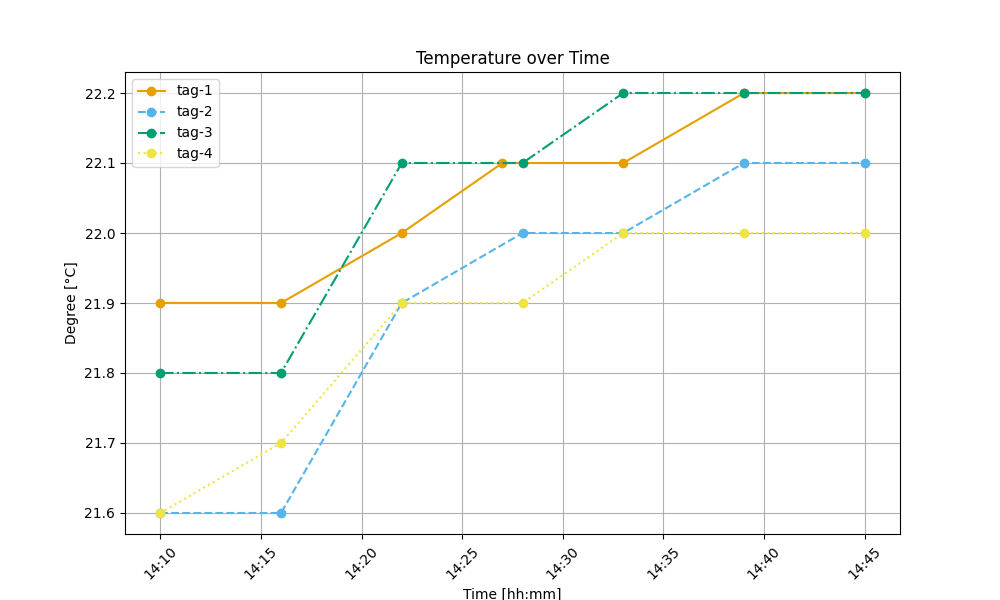
\includegraphics[width=\linewidth]{graphics/exp/exp1_temp_plot_0.png}
	\caption{Experiment 1, temperature over time.}
	\label{f:exp1_graphs_temp}
\end{figure}

Figure \ref{f:exp1_graphs_temp} shows the recorded temperature during experiment 1.
The tags are color coded and use different line-styles.
To make it easier to distinguische the lines, the Y axis only displayes the relevant section, rather then starting at 0\degree .
The time at the bottom represents the timestamp at which the measurement arrived at the phone.
All four tags have a mean temperature between 21.8 and 22.1 \degree C.
The varaince are also small, tag two having the highest one with 0.05 \degree C variance. 
The graph shows that all tags have a rising temperature.
The increase is quite small with tag two having the biggest increase of 0.5 \degree C over 20 minutes.
When the experiment was repeated,, the means stayed similar between the tags and the variance became only smaller.
The trend in temperature changed from upwards to downwards, when the experiment was repeated.

\begin{figure}[ht!]
	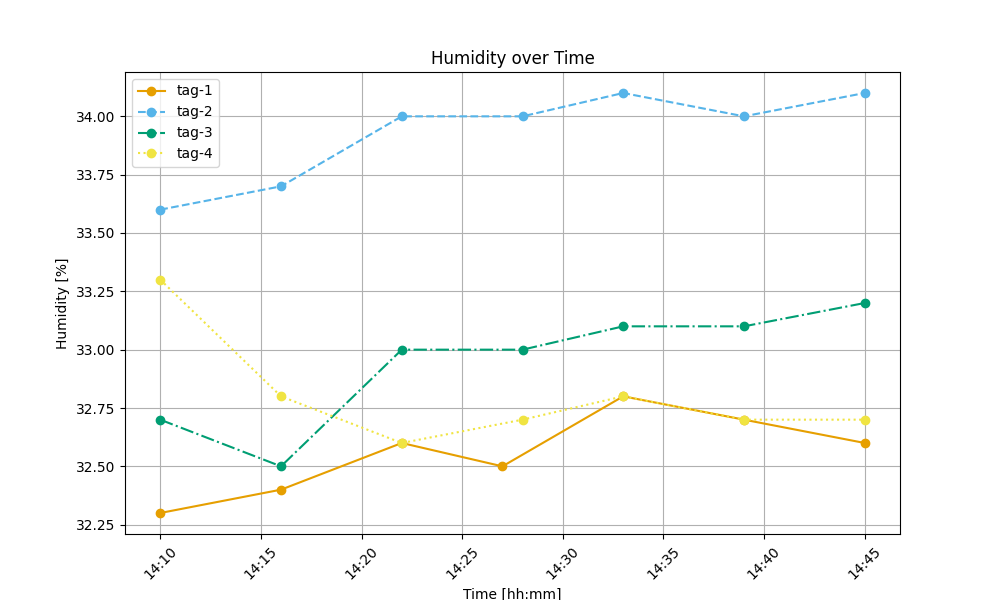
\includegraphics[width=\linewidth]{graphics/exp/exp1_hum_plot_0.png}
	\caption{Experiment 1, humidty over time.}
	\label{f:exp1_graphs_hum}
\end{figure}

Figure \ref{f:exp1_graphs_hum} shows the change of humidity over time.
Again, the relevant section of the y-axis is shown, rather than the full 0\% to 100\% , to increase readability.
The humidity of all sensor was similar as well.
The highest humidity was recorded by Tag-2 with 33.93\% .
Te lowest was recorded by Tag-1 with 32.56\% .
The variance is small, with Tag-3 having the biggest variance with 0.06\% pt.
During the first experiment, humidity increased by a small amount.
When the experiment was repeated,, the humidity dropped during the experiment.


\begin{figure}[ht!]
	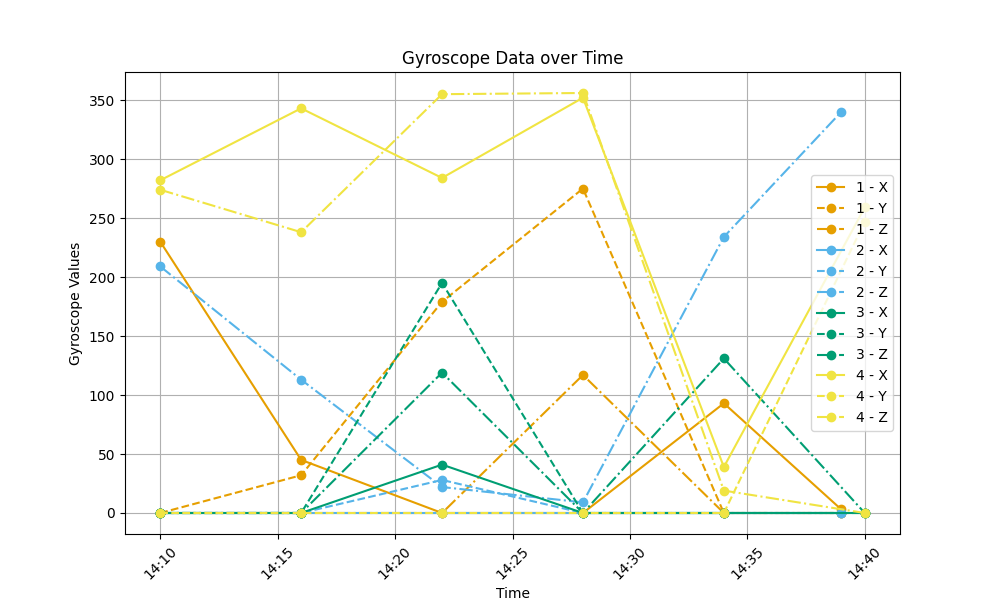
\includegraphics[width=\linewidth]{graphics/exp/exp1_gyro_data_plot_0.png}
	\caption{Registered value of the gyroscope over time during experiment 1.}
	\label{f:exp1_graphs_gyro}
\end{figure}

Since all tags were stationary during the experiment, the gyro sensor was expected to be unchanging.
This is not what occured.
The graph \ref{f:exp1_graphs_gyro} shows the values of the Gyroscope during experiment 1.
Orientational read was used, so the values shoud correspond to the angle around the given axis.
Each tag is assigned a color, and all angle measurements are shown in that color.
All X-axis measurement are diplayed using a filled line.
Axis-Y uses dotted lines.
Point-dotted lines represent the angles around axis-Z
Looking at the graph \ref{f:exp1_graphs_gyro} it is clear, that the measurement shows a wide range of angles for each tag and axis.
The angle of axis-X, Tag-1 (filled orange line) for example, jumps from a value of 230 \degree to 45 \degree, 0 \degree, then stays at 0 \degree for one measurement, goes up to 93 \degree and drops down again to 3 \degree.
As can be seen with this example is, that the measurements also don't fall a clear tragetory.
Tag-1 switches between rising and falling.
The only exception is tag 2 around the x axis, which stays at 0 for the whole measurement duration.\\
Since angle measurements fall into modular arithmetic, it "wrappes around" at 360\degree , means can only meanigfully be taken if the angles are in a small range.
Since this is not the case for most tags, the only mean that is meaningfull is tag 2 axis-x, which has a mean of 0 and a variance 0.

\begin{figure}[ht!]
	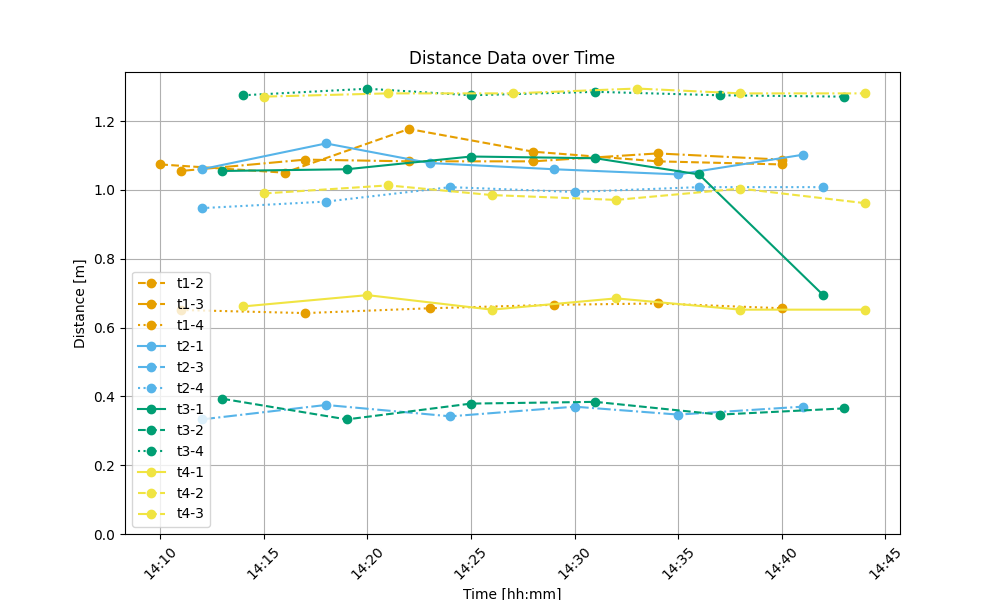
\includegraphics[width=\linewidth]{graphics/exp/exp1_dist_data_plot_0.png}
	\caption{Experiment 1, distance over time.}
	\label{f:exp1_graphs_dist}
\end{figure}

\begin{table}[ht]
\centering
	\caption{Mean, excpected values and variance of distant measurements, experiment 1.}
\begin{minipage}{0.45\textwidth}
	\begin{tabular}{|c|c c c c|}
		\hline
		& \textbf{Tag-1} & \textbf{Tag-2} & \textbf{Tag-3} & \textbf{Tag-4} \\
		\hline
		\textbf{Tag-1} & 0.0 & 1.094 & 1.084 & 0.657 \\
		\textbf{Tag-2} & 1.080 & 0.0 & 0.356 & 0.989 \\
		\textbf{Tag-3} & 1.007 & 0.367 & 0.0 & 1.279 \\
		\textbf{Tag-4} & 0.666 & 0.987 & 1.281 & 0.0 \\
		\hline
	\end{tabular}
	\caption*{Mean}
\end{minipage}
\hfill
\begin{minipage}{0.45\textwidth}
\centering
	\begin{tabular}{|c|c c c c|}
		\hline
		& \textbf{Tag-1} & \textbf{Tag-2} & \textbf{Tag-3} & \textbf{Tag-4} \\
		\hline
		\textbf{Tag-1} & 0.0 & 0.8 & 0.94 & 0.5 \\
		\textbf{Tag-2} & 0.8 & 0.0 & 0.5 & 0.94 \\
		\textbf{Tag-3} & 0.94 & 0.5 & 0.0 & 0.8 \\
		\textbf{Tag-4} & 0.5 & 0.94 & 0.8 & 0.0 \\
		\hline
	\end{tabular}
	\caption*{Excpected values}
\end{minipage}
\hfill
\begin{minipage}{0.45\textwidth}
	\centering
	\begin{tabular}{|c|c c c c|}
		\hline
		& \textbf{Tag-1} & \textbf{Tag-2} & \textbf{Tag-3} & \textbf{Tag-4} \\
		\hline
		\textbf{Tag-1} & 0.0 & 0.002 & 0.000 & 0.000 \\
		\textbf{Tag-2} & 0.001 & 0.0 & 0.000 & 0.001 \\
		\textbf{Tag-3} & 0.024 & 0.001 & 0.0 & 0.000 \\
		\textbf{Tag-4} & 0.000 & 0.000 & 0.000 & 0.0 \\
		\hline
	\end{tabular}
	\caption*{Variance}
\end{minipage}
\label{t:exp1_dist_var}
\end{table}

Table \ref{t:exp1_dist_var}, shows the mean, excpected value and variance of the measured distances.
The tag listed in the row is the queried tag that initiates the distance measurement, and the row corresponding to the responding tag.
By looking to the measurements diagonaly oposed to each other, one can see that the measured distaances is the the same, indipendent of who initiated the measurement, up to a range of two centimeters. 
The measurements from Tag-3 to Tag-1 is the highest, with 0.024m. All other variances are negibly small, beeing bellow 0.005m.
This shows that the measured distances are constant and stable, escept for the measurement from Tag-3 to Tag-1.
The distances measured do not correspond to the actual distances the tags had to each other, also seen in table \ref{t:exp1_dist_means}.
The measured distances can be as far of as 0.5 meters.
The two larger distances, 0.8 and 0.94 meters, correspond to the two larger measured values for each tag, while the smallest measured value always corresponds to the smallest distance, 0.5 meters.
The two larger values are not always ordered correctly, 0.94 meters sometimes beeing measured smaller then 0.8 meters.
In repeated experiments, all these facts stayed true.


Figure  \ref{f:exp1_graphs_dist} shows the measured distance over time.
A label i-j informe that tag-i initiated the measurement, and the distance between tag-i and tag-j was measured.
All measurements initiated by Tag-1 are orange. The meausrements of Tag-2 are blue, Tag-3 green and Tag-4 yellow.
The second tag that is involved in the measurement is signified by the line.
Measurements to Tag-1 use filled lines. Measurements to Tag-2 use dashed lines, Tag-3 uses dashed and dotted lines and Tag-4 uses dotted lines.\\
All lines except for 3-1 are horizontal  and show little variance.
Measurement 3-1 is also stable untl the last measurement, where a datapoint that is 0.35m lower than all previously recorded data is measured.
One can also see that not all measurements start at the same time.
The first measurement of distance 1-2 was registered at 14.10, while the first measurement of 4-3 was recorded at 14.15.
Each distance was measured seven times and with equidistance measurement times.

\begin{figure}[ht!]
	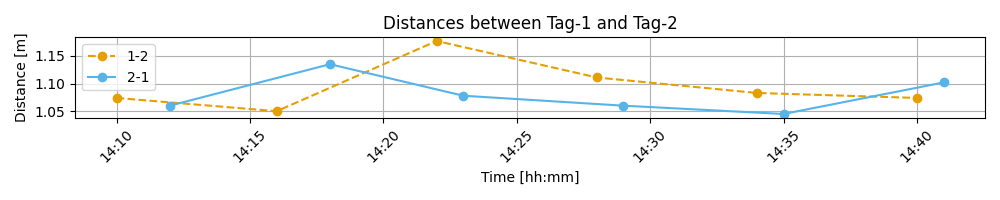
\includegraphics[width=\linewidth]{graphics/exp/exp1_dist_data_plot_1_1_2_split.png}
	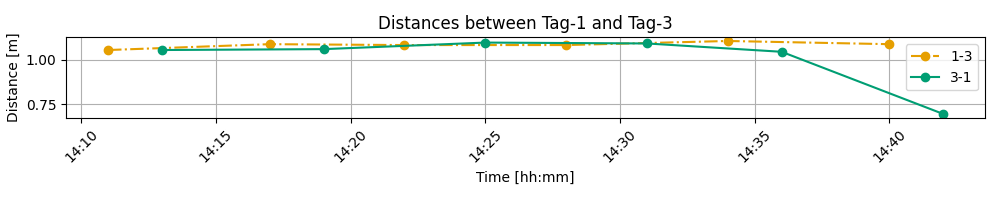
\includegraphics[width=\linewidth]{graphics/exp/exp1_dist_data_plot_1_1_3_split.png}
	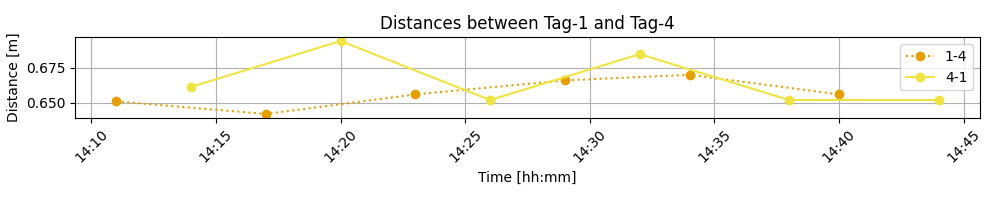
\includegraphics[width=\linewidth]{graphics/exp/exp1_dist_data_plot_1_1_4_split.png}
	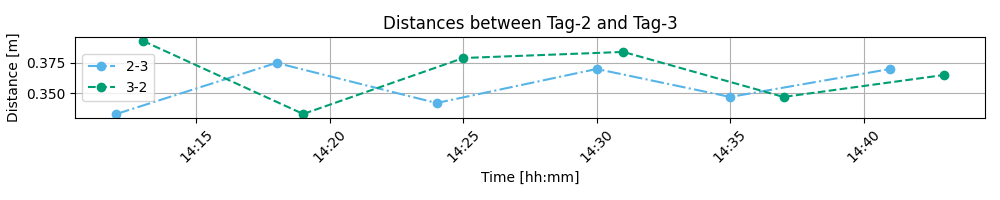
\includegraphics[width=\linewidth]{graphics/exp/exp1_dist_data_plot_1_2_3_split.png}
	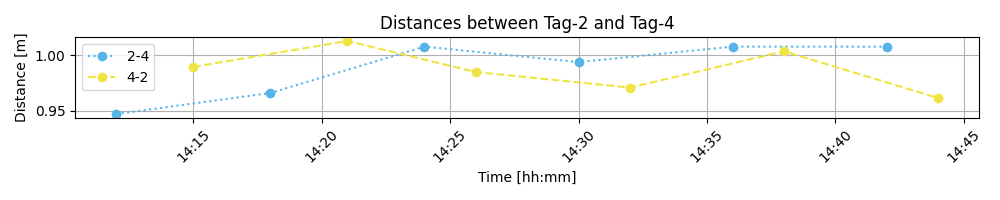
\includegraphics[width=\linewidth]{graphics/exp/exp1_dist_data_plot_1_2_4_split.png}
	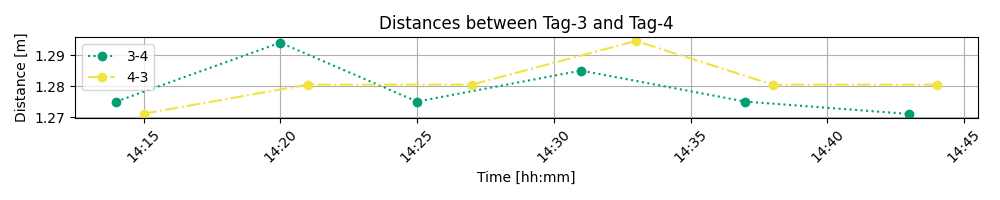
\includegraphics[width=\linewidth]{graphics/exp/exp1_dist_data_plot_1_3_4_split.png}
	\caption{Experiment 1, distance over time, for all pairs i-j.}
	\label{f:exp1_graphs_dist_split}
\end{figure}


The measurement pairs i-j and j-i report the same distance, but with different tags initiating the measurement. 
To better compare these pairs, figure \ref{f:exp1_graphs_dist_split} shows six subplots of figure \ref{f:exp1_graphs_dist} containing only each of these pairs.
The graphs show that the measurement pairs anre consistently close together.
One outlier happens when Tag-3 measures the distance to Tag-1 at very end of the measurements.
The measured value drops 0.35m bellow the previous mean of 1.30m.
When repeating this experiment and during other experiments, these outliers happened again, a bit less frequently then twice per hour.
The outliers always affected a measurement involving tag 1.

\begin{figure}[ht!]
	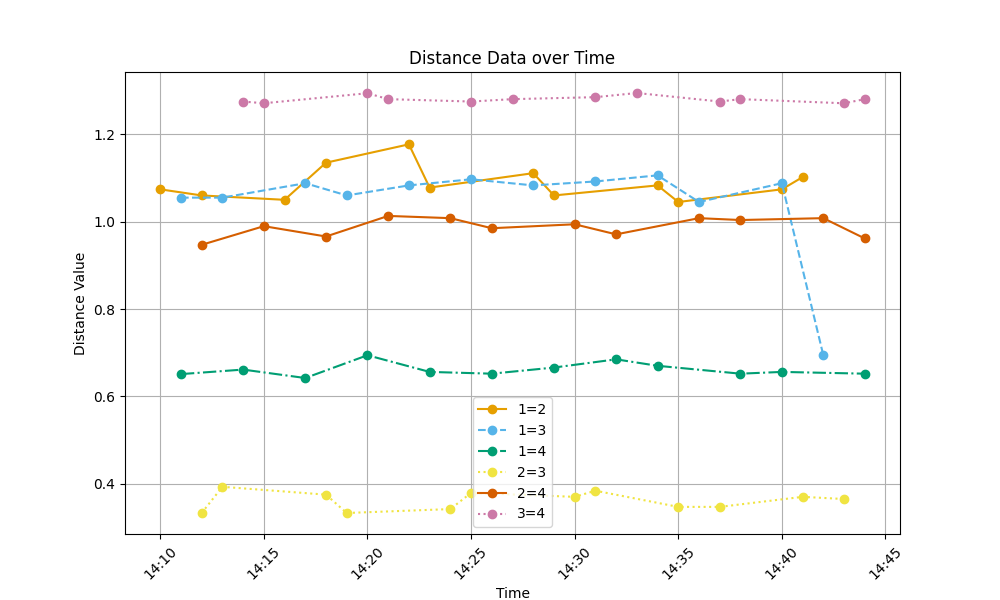
\includegraphics[width=\linewidth]{graphics/exp/exp1_dist_data_plot_1_combined.png}
	\caption{Experiment 1, distance over time, for comined pairs i=j.}
	\label{f:exp1_graphs_dist_combined}
\end{figure}

Since the pairs i-j and j-i report the same data and this fact is consistent in the measurements, they can be combined into one graph.
Figure \ref{f:exp1_graphs_dist_combined} shows the distances over time for all combined pairs i-j and j-i, called i==j.
Graphs like this will be called combined graphs in this report.
Since initiating and reseiving tag can no longer be distinguished, the line colors and types have no assigned meaning.
The two pairs 2=3 and 1=4 corresponding to the two low distances of 0.5m can be seen at the bottom.
The pairs 1=3 and 2=4 that represent the highest distance of 0.94m do not separate and are mixed together with 1=2 and 3=4.\\
Table \ref{tab:exp1_var_distanc} shows the means and variances of the combined tag pairs.
Since the measurements of i=j are the same as j=i, only the upper triangle of the distance-matrix is needed.
The table shows, that the variances are very low for all pairs, except 1=3.

\begin{table}[ht]
\centering
\caption{Statistics of the combined distance measurements between tags for experiment 1}
\begin{minipage}{0.45\textwidth}
\centering
\begin{tabular}{|c|c c c|}
\hline
		& \textbf{Tag-2} & \textbf{Tag-3} & \textbf{Tag-4} \\
\hline
\textbf{Tag-1}    & 0.112 & 0.265 & 0.177 \\
\textbf{Tag-2}   &  & 0.368 & 0.824 \\
\textbf{Tag-3}   &  &  & 0.385 \\
\hline
\end{tabular}
\caption*{Mean}
\end{minipage}
\hfill
\begin{minipage}{0.45\textwidth}
\centering
\begin{tabular}{|c|c c c|}
\hline
		& \textbf{Tag-2} & \textbf{Tag-3} & \textbf{Tag-4} \\
\hline
\textbf{Tag-1}    & 0.001 & 0.013 & 0.000 \\
\textbf{Tag-2}   &  & 0.000 & 0.000 \\
\textbf{Tag-3}   &  &  & 0.000 \\
\hline
\end{tabular}
\caption*{Variance}
\end{minipage}
\label{tab:exp1_var_distanc}
\end{table}


\subsection{Conclusion}
\label{s:exp1_conclustion}
The temperature measurement seem to be working as excpected.
All four tags show the same temperature, within a small margin of error.
Variance is low, showing a consistent temperature measurement.\\
Two possible explenations were found for the increase in temperature during the experiment.
One possible explenation is given by the fact, that this was the first experiment performed in the day, and the room temperature was slightly increasing because of the presence of a person, that was not present before.
An alternative explenation is, that the microprocessors proucde heat that was detected.
The fact that the temperature decreased during subsequent experiments, favors explenation one, since their would be no reason for the microcontrolers to stop producing heat.
The decrease itself can be explained, since during setup, the person performing the experiment was close to the sensor, while during the experiment the person stayed in a different part of the room. The dicrease in temperature was smaller, this difference in closness to body heat could explain the difference.


The humidity sensor similarly produced satisfactory results.
All four tags presented the same humidity, only with small margins of error.
The variance is again satisfactory, since it is very small, beeing bellow 0.05%.
The slight increase in humidity can again be explained by this beeing the first experiment of the day, and the person performing the experiment having wet hair from the rain.
This again weakenes the microcontoler heat theory, since rising temperature without adding moisture would only decrease the humidity.\\
The dicrease in humidity in subsequent experiments lacks a clear explenation.
It is a very weak trend, so factors global factors could explain the difference.
Changing weather conditions could account for the difference.
Another proposed explenation arises from the setup of the system.
During setup, each tag was touched repeatedly to put them into position.
The person performing the experiment tends to have clamy hands, that feasably could lead the sensors to detect additional humidity at the beginning of the experiment.\\
Without additional data, no one explenation can be favored over the other. 
Since the decrease in temperature was small, this is not considered a issue for this system.


The Gyroscoping sensor data does not produce any meaningfull result.
The measured orientation of the tags varied widely, while the physical tags stood still.
A possible explenation of this is, that the gyroscope used in the implementation has consistent biases.
Since the angular velocity is evaluated often and then added to the current angle, small errors would acumulate over time.
The time between measurements was 5 minutes and 30 seconds.
A bias of only $\frac{12}{11} \frac{\degreem}{s}$ would correspond to an accumulated error of 360\degree over this timespan.
Since rotational position in inheritly circular, rapping arround at 360 \degree, unless there was no variance next to the bias, the values would end sudo randomly scattered over the range of $[0\degreem , 360\degreem ]$.
The MPU6050 outpus only integers, so any bias at all would have this effect.\\
Be bias hypothoses is additionaly strengthend, by the existance of Tag-2 axis X, that stays at 0 over the course of the measurement.
While this could indicate a faulty sensor, during later experiments using rotational velocity readings, see section\ref{s:exp_5_real_world}, Tag-2 axis X did produce meaningfull results. While this doesn't disproove, that Tag-2 axis X was faulty during this experiment, it makes it more reasonable to assume, that it has a bias of 0. \\
A possible reason for the bias in angular velocity was considered, in the rotation of the earth.
After some consideration, this thesis was dropped, since the angular velocity introduced by the earth would acount for no more than $\frac{1}{240} \frac{\degreem}{s}$ around the X or Y axis, if standing on the equator, where the effect is strongest.\\
The bias explenation seems to be a reasonable and explaines the measured results.
As a consequence, the orientational read has to be considered usless.


The distance measurements have mixed results.
The fact that the tag pairs produce the same same reults is good.
Double sided two-way ranging is used, so during each ranging session both tags conduct single-sided two-way ranging and the results are combined.
It is therefore expected, that the device that initiates the ranging does not matter.\\
The fact that ranging sessions involving Tag-1 occasionaly produce inconsistent results can not directly be explained.
Different locations were used for the experiments and the tags did not always have the same position.
This means that an explanation envolving multi-path effect based on position can be rejected.
The possible explenation envolves a fault on the nRF52840 microcontroler or the DMW3000 shield. 
Since the final calculation relies on the timestamps recorded during the ranging, a possible explenation would be, that the clock of the nRF52840 sometimes faults, or that there is an issue with the clock line of the SPI connection.\\
The fact that the resulting distances are wrong is troublesome.
The proposed design that would calculate the position by solving a quadratic program relies on somewhat accurate distance measurements.
The likely reason for the distance measurements producing wrong results is the simplified calibration, that was used for the $d_{rx}$, $d_{tx}$ values, see Section \ref{ss:two_way_ranging}.
The fact that the distances still sort themself into high and low values correctly indicates, that some calibration has worked, but it is not granular enough to work for small distances.\\
The distance measurements can currently not be used to build a model of the tag positions.
If they can be used to detect movement can not be determined by the static experiment and requires the introduction of movement, see Experiment 4 \ref{s:exp4}


\section{Experiment 2: Temperature}
\label{ss:exp_2}

\begin{figure}[ht!]
	\centering
	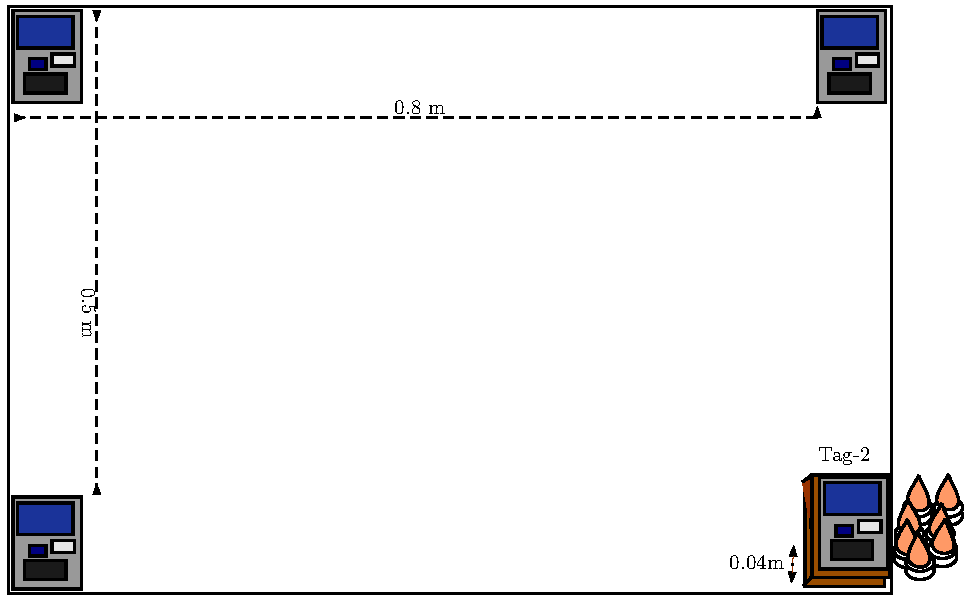
\includegraphics[width=300px]{graphics/schematics/experiment_2.pdf}
	\caption{Schema of the setup of experiment 2.}
	\label{f:exp2_schematic}
\end{figure}


The four tags were placed in the same 80 cm by 50 cm rectangle as in experiment one.
One tag placed on a elevated surface, 4 cm above the table.
next to the tag on the table, seven candles were placed (see figure \ref{f:exp2_photo} ).
Next to the Tag-2 thermometers detectors were placed.
Figure \ref{f:exp2_schematic} shows a schematic view of the setup.
Each tag was turned on sequentially and given enough time to establish the network.
The phone then was connected to one tag.
The max Temperature parameter in the app was changed to 35\degree C.
After 20 minutes the candles were lit.
The experiment was then left alone for another 30 minutes.
The independent thermometers were filmed during the process, to allow for later review and comparesment.
The goal of experiment 2 was to test the temperature detection capabilities of the system.

\begin{figure}[ht!]
	\centering
	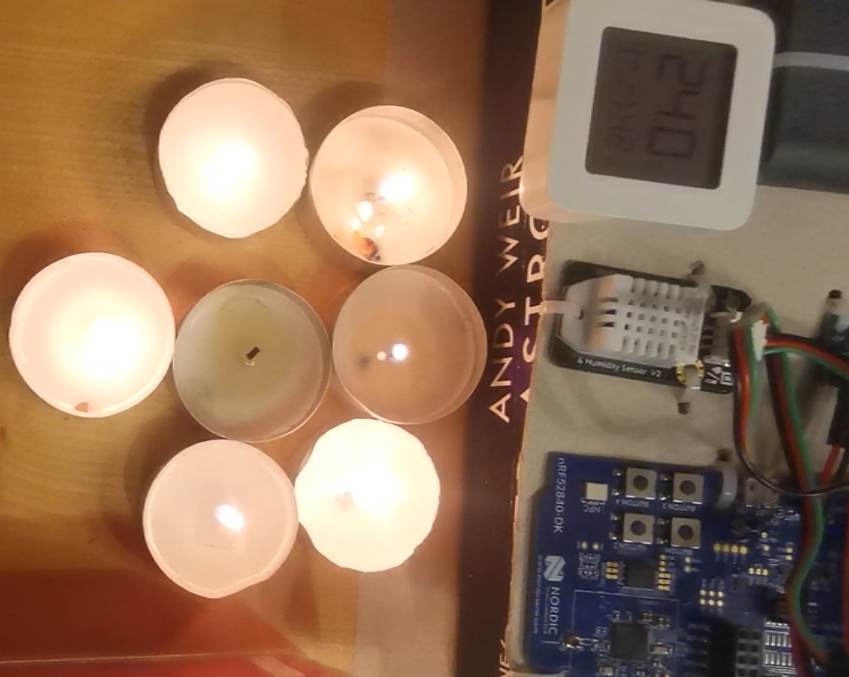
\includegraphics[width=300px]{graphics/exp/Exp_2_photo.png}
	\caption{Photo of elevated Tag-2, candles and thermoeter used in experiment 2.}
	\label{f:exp2_photo}
\end{figure}


\subsection{Results}
\label{ss:exp_2_result}
Experiment two introduced heat-sources to the system.
Since the main setup was the same as experiment 1 \ref{ss:exp_1_result}, many of the findings are the same.
In this section, only differences in results are discussed.
If a metric is not measioned, one can assume it behaved the same as for experiment 1  (see section \ref{ss:exp_1_result}).

\begin{figure}[ht!]
	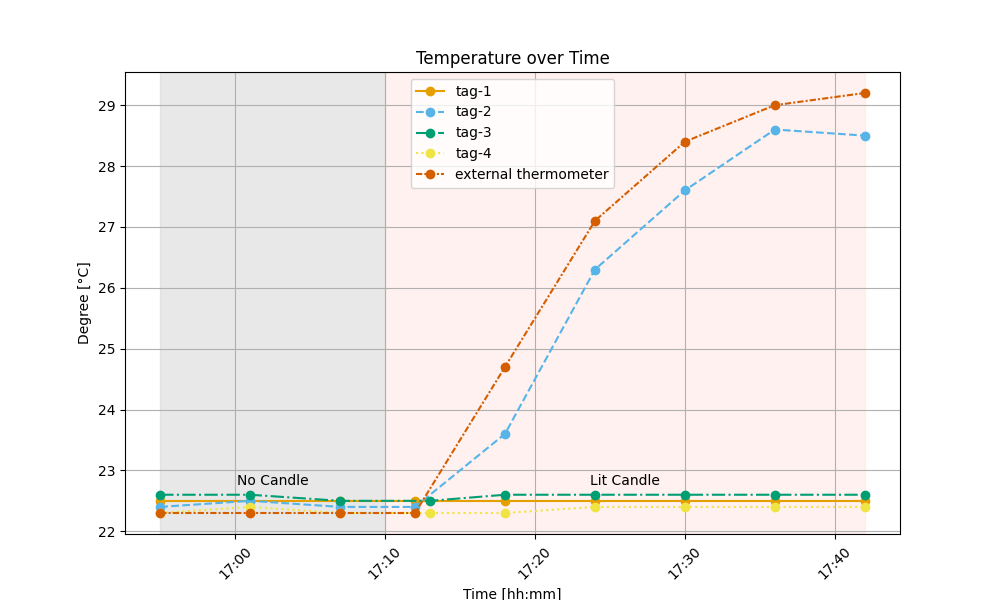
\includegraphics[width=\linewidth]{graphics/exp/exp3_temp_plot_1.png}
	\caption{Experiment 3, temperature over time, mith external measurement added.}
	\label{f:exp3_graphs_temp}
\end{figure}

The progression of the external thermoeter and the internal temperature sensor can be seen in figure \ref{f:exp3_graphs}.
The candles, that functioned as the heat source, were lit at 15.10.
The section of time before the candle was lit has a gray background.
After the candle was lit, the background becomes red.
The measurements from te external thermometor are shown with a red dashed and dotted line.
They were extracted manualy from the video. The datapoints correspond to the datapoints when Tag-2 measured.\\
Before the candle was lit, Tag-1, Tag-2, Tag-3 and Tag-4 recorded mean temperatures of 22.5\degree C, 22.4 \degree C, 22.6 \degree C and 22.3 \degree C respecivly.
The variances were all bellow 0.01\degree.
Once the candle was lit, Tag-1, Tag-3 and Tag-4 continued with similar temperature, havin mean temperatures of 22.5\degree C, 22.6\degree C and 22.4\degree C over the whole duration, with variance remaining under 0.01\degree C.


After the canle was lit, Tag-2 started to deviate from the other tags.
During the next measurement of tag 2, at 15.12, both the external thermoeter and the temperature sensor on tag 2 had not yet registered any change, remaing at 22.4 \degree C for the tag and 22.3 \degree C for the external thermometer.
The recording showed the extrenal thermometer start rising 1 minutes later, at 15.13.
During the next measurement at 15.18, the temperature-sensor registered a slightly increased temperature of 23.6 \degree C, while the external thermometer registered 24.7 \degree C.
During the next measurement at 17.24 the tag reported 26.3 \degree C while the thermometer showed 27.1 \degree C. 
The measured temperature of the external thermometer keeps klimbing faster than the temperature sensor of Tag-2, until the end of the experiment, as seen in Figure \ref{f:exp3_graphs_temp}.
The difference in measured temperature between Tag-2 and the external thermoeter nether exeeds 1 \degree C and gets smaller towards the end of the experiment, ending with a difference of 0.7 \degree C.

\begin{figure}[ht!]
	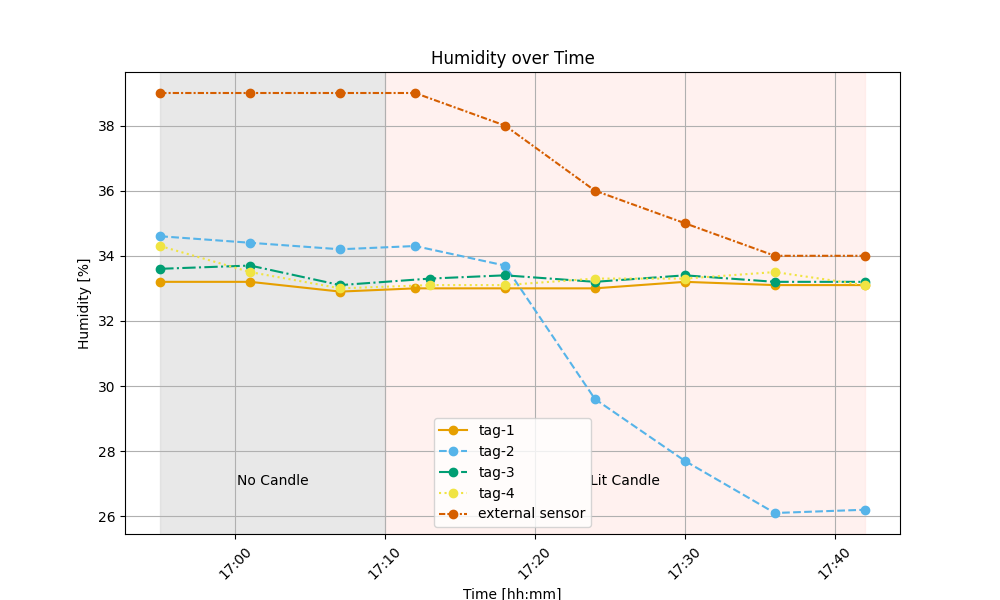
\includegraphics[width=\linewidth]{graphics/exp/exp3_hum_plot_1.png}
	\caption{Experiment 3, humidity over time, with external measurement added.}
	\label{f:exp3_graphs_hum}
\end{figure}


Experiment 3 was intended to test the temperature and not the humidity.
Luckily, the external thermoeter also included a humidity sensor, that could retroactivly be used for evaluation.
Figure \ref{f:exp3_graphs_hum} shows the humidity over time,the gray and red sections again representing the time before and after the candle was lit.
The external humidity sensor wasa added to the graph and is shown with a red dashed and dotted line.
Since the external humidity sensor was initialy not intended to be used, it is not perticulalry precise and does not display any digits after the decimal point.\\
Its values were again manual extracted from the video at the same points the times Tag-2 measured the humidity.
Tag-1, Tag-3 and Tag-4 again show a constant measurement during the experiment, having mean humidities of 33.0\% , 33.3\% and 33.4\% .
Tag 4 has the highest variance of the group, with 0.2\% , the others havin variances bellow 0.1 \%.\\
Tag-2 had a higher mean humidity of 34.4 before the candles were lit, with a variance of 0.04.
The first measurement after the candle was lit was still 34.3 \% . Afterwards the measurements started dropping, first with a small dicrease to 33.7 \% , followed by a large drop to 29.6 \%, then 22.7 \% and finally platoing at 26.2 \% .\\
The humidity sensor consitently shows a much higher humidity than the one on the tag.
When the experiment starts at 15.10, the external sensor shows a humidity of 39 \% .
It stays on this value until the candle is lit.
The first measurement after the candle is lit, at 17.12 still has a humidity of 39\% .
The external sensor than first notes a small dicline of 1\% pt, followed by a larger decline of 2\% pt to 36 \% and then decends with 1\% pt at a time until it platoes at 34\% . \\
The humdity registered by Tag-2 and the external sensor forms a similar line.
This two lines have a similar tragectory, but are not parallel.
While the difference in registerd humidity originaly is around 4.6\% pts, when both platoe, the difference has risten to 7.8\% pts.
The variance in the difference of the Tag-2 sensor and the external sensor is 2.1 \% pts over the whole measurement period.

\subsection{Conclusion}
The fact that the three sensors that are far away from the sensor don't show any sign of temperature increase was expected.
Since warm air rises, and the tags were spread more than half a meter apart, it was not expected, that the heat from the candles would reach the tags.
Even if hot air would nor rise, the energy added to the system would  be added with an efficiency of $\mathbf{O}(d^{\frac{1}{3}})$, where d is the distance.\\
The tag that is close to the candle does notice the candle with a similar speed as the external thermoetor.
The fact that it takes a while for both the external sensor as well as the sensor of Tag-2 to register the heat, has two explenations.
The first explenation is, that the external thermoetor and the DHT22 sensor are both not high precision instruments and have a natural inertia.
The second explenation is, that it takes a moment for the candles to fully burn and start heating up the air.
most likely, a combination of both factors is responsible for the delayed start.\\
The obervation that the external thermoetor registeres a higher heat than the internal sensor has two possible explenations.
It could be a difference in registered value, due to different sensor reporting different results.
It could also be, that the external sensor was actually hotter than the internal sensor.
The internal sensor was mounted on a piece of cardboard and thus shielded a bit from the heat.
The external sensor was also placed on the cardboard, but more directly exposed to the heat, sine it was placed closer to the edge of the cardboard piece.
Since initialy both sensor have very similar values, the second explenation is mire likely true.


The fact that the humidity dropped when the candles were lit should have been expected.
The \% humidity represents amount of water in the air, as a percentage of the maximal capacity of air.
The capacity of air to carry water rises with temperature.
So when the temperature rises, but no additional humidity is added, the percentage drops.
This can clearly be seen happening in this experiment to Tag-2.\\
Since the temperature around Tag-1, Tag-3 and Tag-4 does not rise, neither does the humidity fall.
This was verified by the humidity results of this experiment for those tags.\\
Tag-2 startes with a slightly increased humidity.
This is a further pointer to the theory, that the humidity of the experimenter during setup can be registered, since it took the experimenter a few minutes to set up everything around Tag-2 for experiment 2. \\
The difference in humidity between the tags and the external sensor lacks a clear explenation.
Since the humidity function is not the main purpose of the external thermometor, it is possible that it was implemented poorly, thus leading to the difference.
Further research is required to analize the precision of the DHT22 sensors.
Nethertheless, the sensor on Tag-2 shows clearly a happening thenomenon, indicating that the gerneal implementation and setup is soudn.



\section{Experiment 3: Gyroscope}
\label{s:exp_3}
Again all for tags were placed on a 80 cm by 50 cm rectangle.
Each tag was turned on sequentially and given enough time to establish the network.
The phone then was connected to one tag.
After 20 minutes one tag was turned by 90\degree clockwise.
The experiment then ran for another 30 minutes.
The goal of experiment number 4 was to test the detection of unwanted rotations.


Experiment 3 was performed in two differing manners.
The orirentational read was originaly the only implementation for the gyroscope.
After experiments one to four were evaluated, the lack of usefull results from the gyroscope readings prompted a redesign of the sensor.
This resulted in the development and implementaiton of the angular velocity read.
Experiment 3 was repeated with the angular velocity read of the gyro.\\
For the orientational read, the maximal allowed angular difference was set to 30\degree.
For the angular velocity read, the maximal allowed angular velocity was set to 100 $\frac{\deg}{s}$.
The results for the orientational and the angular velocity read will be presented seperatly. The conclusion will talk about them both.


\begin{figure}[ht!]
	\centering
	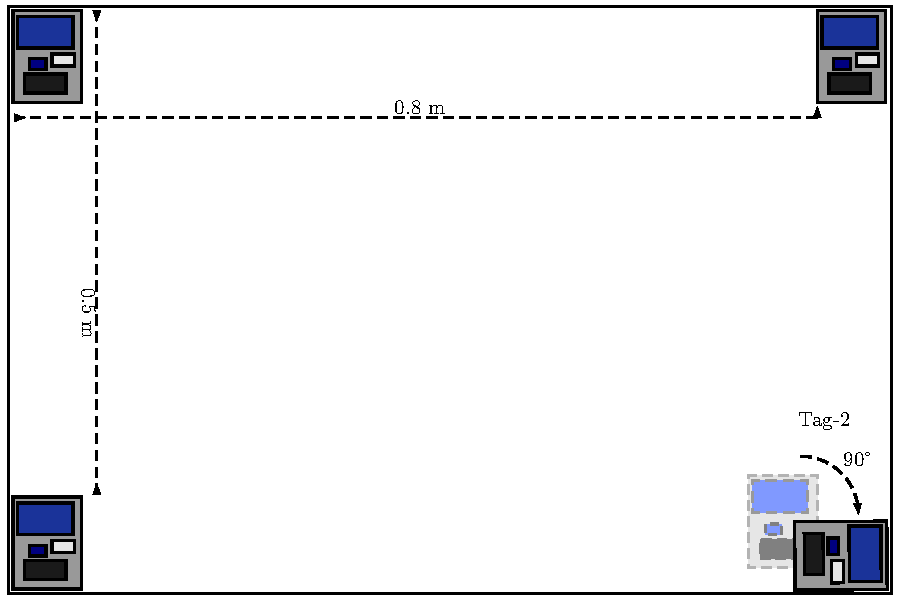
\includegraphics[width=300px]{graphics/schematics/experiment_3.pdf}
	\caption{Schema of the setup of experiment 3.}
	\label{f:exp3_schematic}
\end{figure}


\subsection{Reults orientational read}
\label{ss:exp_3_result}
Experiment 3 was intended to check the functionality of the gyroscope.
Temperature and humidity behaviour were the same as in the static experiment \ref{ss:exp_1_result}.
As already seen during the evaluation of experiment 1, the gyroscope does not work as planned.


Figure \ref{f:exp4_graphs_gyro} shows the values of the gyro over time.
Tag 1 was rotated by 90\degree  at 22.25 around the Z axis.
The gray section marks the park of the experiment beofre the turn, while the red shows the results after the turn. \\
Tag-3 has a mean of 0 and 0 variance of 0 during the whole experiment for axes X and Y.
Tag-4 has one measurement that has 0 mean and variance as well, at axes Y.
Their is no disernable change in the output of the gyro during or after this process in any of these measurements. \\
Some other orientation are also manly zero during this experiment.
The orientation of the Z-Axis of Tag-3 is zero for six out of the eight performed measurements, only spiking once at the beginning for two reads.
The other axes of Tag-1 have values 100\degree and 290\degree at the beginning and then stay zero for the rest of the experiment.
The Y and Z axis of Tag-2 are also zero for almost all measurements except for one measurement at 22:11, where they registered an orientation of 235\degree and 5\degree respecivly
This is escpecially unescpected, since Tag-2 was the one who was turned around axis Z. \\
Axis z of Tag-1 forms zig-tag line between values from 25\degree to 100 \degree and 200 \degree to 300 \degree.
Tag-4 axis X and Z and Tag-2 Axis X follow no decernable pattern.


\begin{figure}[ht!]
	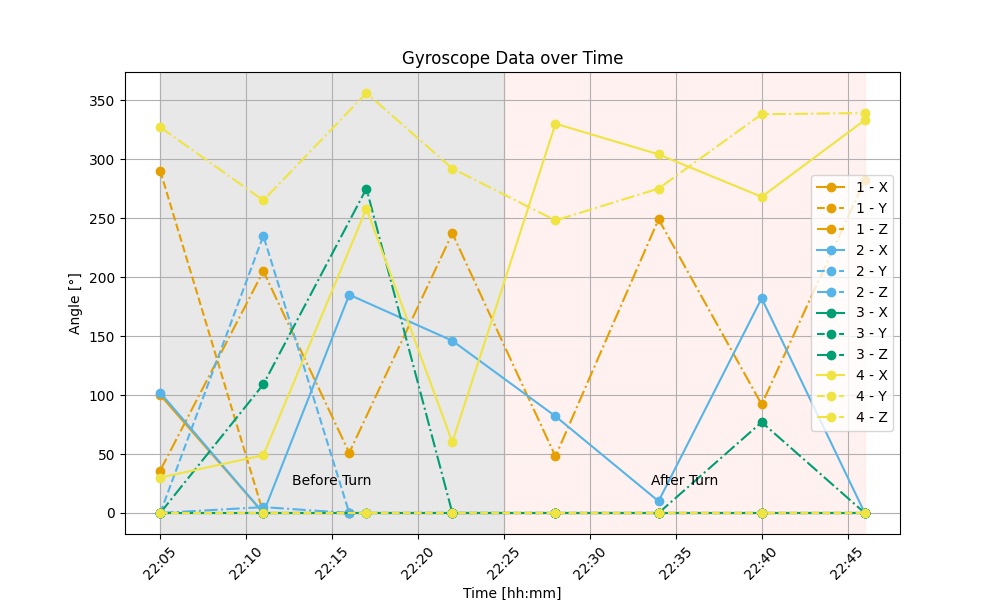
\includegraphics[width=\linewidth]{graphics/exp/exp4_gyro_data_plot_1.png}
	\caption{Experiment 4, gyroscope over time.}
	\label{f:exp4_graphs_gyro}
\end{figure}

Figure \ref{f:exp4_graphs_dist} shows the distances over time for pairs, as discussed in section \ref{ss:exp_1_result}.
Before the event, all measured distances are stable, except for one outlier in the distance 1=2.
As in experiment 1 \ref{ss:exp_1_result} the distances are not equivalent with the physical distances in the experiment.\\
After the tag is turned at 22.26, all measurements involving Tag-2 change and then remain at the new distance.
Distance 1=2 dicreases from 0.71 m to 0.42, after a short jump to 1.4m.
Distance 2=3 is on 0.92 before the measurement and 1.11m afterwards. It is also involved in a measurement during the turn, measuring 0.65m.
Distance 2=4 is originaly at 0.65m before the turn and ends up at 1.10m afterwards.
The other pairs, 1=3, 1=4 and 3=4 don't change values siginificantly during this time, having variances of 0.001, 0.004 and 0.000 respectifly.

\begin{figure}[ht!]
	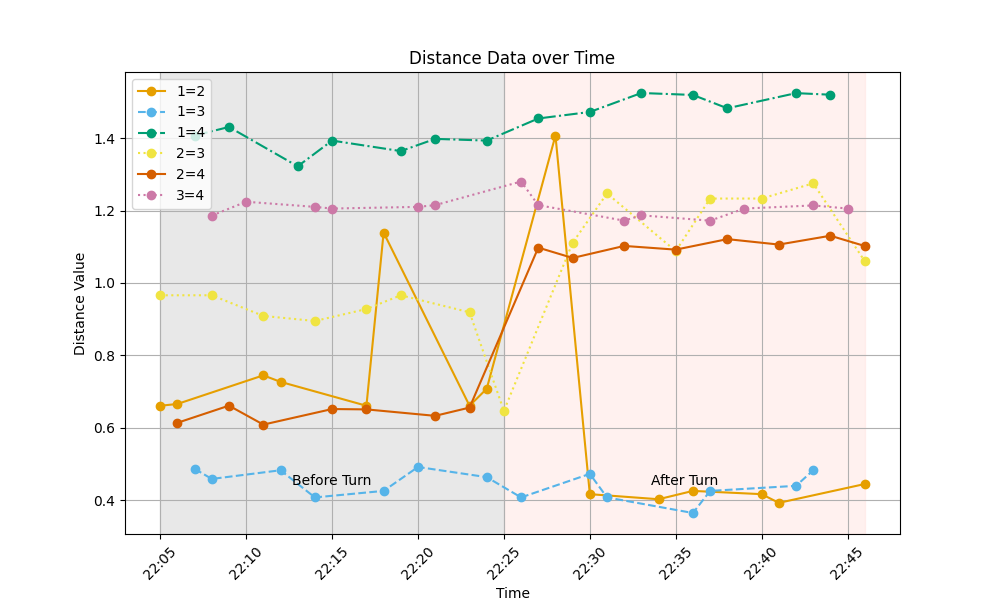
\includegraphics[width=\linewidth]{graphics/exp/exp4_dist_data_plot_1.png}
	\caption{Experiment 3, gyroscope over time.}
	\label{f:exp4_graphs_dist}
\end{figure}


\subsection{Results angular velocity read}
\label{ss:exp_3_result}
As with the orientational read, this experiment had no results that differed from the static experiment, when analyzing temperature and humidity.
The experiment was started at 10:01 and was terminated 10.40.
Tag 2 was turned at 10.18 by 90\degree around the Y axis by hand.
Figure \ref{f:exp4_graphs_gyro_2} shows the angualr velocity of all tags during the experiment.
The angular velocity of tag i around axis v will be labeled as $a_i^v$.
All axises of Tag-2 are shown in blue, with the angular velocity around the X axis, $a_1^X$ ,beeing a filled line, around the Y-Axis a dashed line and around the Z axis beeing dashed and dotted.
The Y axis of figure\ref{f:exp4_graphs_gyro_2} is displayed using a log-scale, to better show the low values.
The time before the utrn has a gray backgroudn, while the time after the turn is displayed with a red background.


Tag-2 has constant angular velocity for all three measurements before the turn.
$a_2^X$ is $12\frac{\degreem}{s}$, $a_2^Y$ is between $14\frac{\degreem}{s}$ and $17\frac{\degreem}{s}$  and $a_2^Z$ is a constant $20\frac{\degreem}{s}$ before the turn.
The first measurement after the turn reports angular velocities of $445\frac{\degreem}{s}$, $6322\frac{\degreem}{s}$ and $716\frac{\degreem}{s}$ for axis X,Y and Z of Tag-2.
Afterwards the values return back to their original values.
$a_2^X$ is $13\frac{\degreem}{s}$, $a_2^Y$ is $14\frac{\degreem}{s}$ and $a_2^Z$ $20\frac{\degreem}{s}$, all constant measurements, after the turn.

\begin{figure}[ht!]
	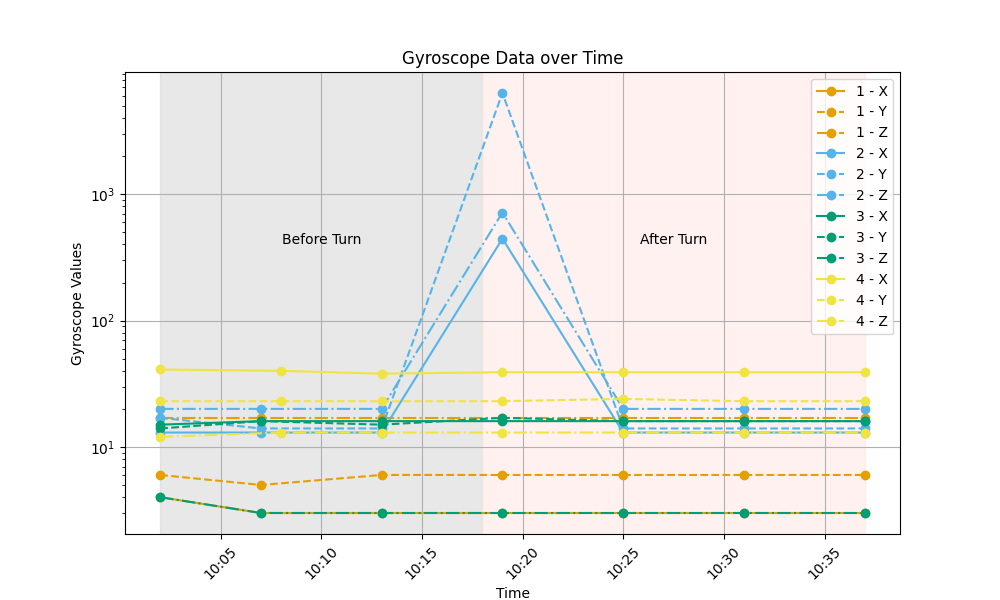
\includegraphics[width=\linewidth]{graphics/exp/exp4_2_gyro_data_plot_2.png}
	\caption{Experiment 3, gyroscope over time, using the angular velocity read.}
	\label{f:exp4_graphs_gyro_2}
\end{figure}

Tag-1, Tag-3 and Tag-4 are in orange, green and yellow respectivly.
They all keep a measurements with minimal fluctuation.
Table \ref{tab:gyro_mean_2} shows the mean values and variances of all tags and all axes.
Tags-1 has no variance that exceeds 0.143, with $a_1^Z$ even showing a constant value over all seven measurements, leading to a variance of zero.
Tag-3 and Tag-4 both have two axes with variances of 0.143 and one axis with a variance of 0.905.
The mean values of Tag-1, Tag-3 and Tag-4 are in the reange of $3\frac{\degreem}{s}$ and $40\frac{\degreem}{s}$, with five falling into the range of $15\frac{\degreem}{s}$ to $25\frac{\degreem}{s}$.
Tag-2 has variances between 740 and 16128.

\begin{table}[h!]
\centering
\caption{Summary of Gyroscope Data: Means and Variances of X, Y, Z Axes}
\begin{tabular}{c|c c c|c c c|}
\hline
\textbf{tag} & \textbf{mean x} & \textbf{mean y} & \textbf{mean z} & \textbf{var x} & \textbf{var y} & \textbf{var z} \\
\hline
\textbf{tag-1} & 3.143 & 5.857 & 17.000 & 0.143 & 0.143 & 0.000 \\
\textbf{tag-2} & 23.3 & 41.3 & 68.0 & 741 & 5024 & 16128 \\
\textbf{tag-3} & 15.857 & 15.714 & 3.143 & 0.143 & 0.905 & 0.143 \\
\textbf{tag-4} & 39.286 & 23.143 & 12.857 & 0.905 & 0.143 & 0.143 \\
\hline
\end{tabular}
\label{tab:gyro_mean_2}
\end{table}


Figure \ref{f:exp4_graphs_dist_comb_2} shows the pairs of ditances over time of experiment 3 using angualr velocity read.
The distances 1=2, 1=3, 1=4, 2=3 and 2=4 stay in a similar range over the whole experiment.
Table \ref{tab:exp4_var_distanc} shows the mean and variance of the combined distance measurements.
The variance in measured distances 1=2, 1=3, 1=4, 2=3 and 2=4  are all below one milimeter.
The measured distances are between 0.39m and 0.87m.
The measured distance 3-4 behaves very differently.
It is bigger than all others, with 1.18m.
It also has a comperatavly high variance of 0.05m.
Its lowest measurement is the first measurement after the turn.
Looking at the split distance-measurement 3-4 in figure \ref{f:exp4_graphs_dist_split_3_4} shows, that the change in distance comes mainly from the measurements originating from tag 3.
Distance measurements from Tag-3 to Tag-4 have a variance of 0.074m, while measurements from Tag-4 to Tag-3 have a variance of 0.014m.

\begin{figure}[ht!]
	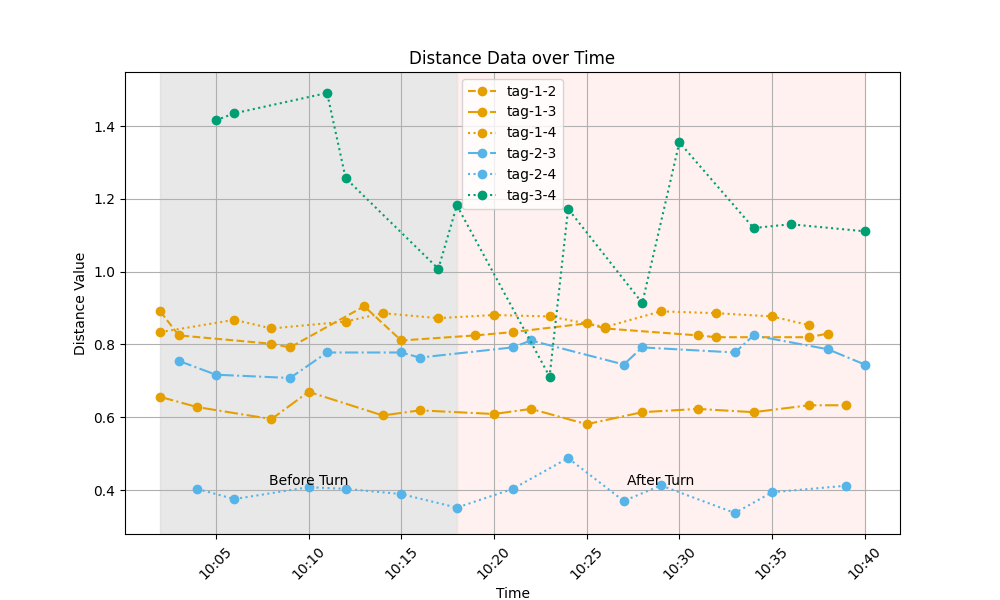
\includegraphics[width=\linewidth]{graphics/exp/exp4_2_dist_combined_2.png}
	\caption{Experiment 3, combined distance over time, using angular velocity read.}
	\label{f:exp4_graphs_dist_comb_2}
\end{figure}

\begin{table}[ht]
\centering
\caption{Statistics of the combined distance measurements between tags for experiment 3 with angular velocity read}
\begin{minipage}{0.45\textwidth}
\centering
\begin{tabular}{|c|c c c|}
\hline
  & 2 & 3 & 4 \\
\hline
1    & 0.0.834 & 0.622 & 0.868 \\
2   &  & 0.770 & 0.396 \\
3   &  &  & 1.177 \\
\hline
\end{tabular}
\caption*{Mean}
\end{minipage}
\hfill
\begin{minipage}{0.45\textwidth}
\centering
\begin{tabular}{|c|c c c|}
\hline
  & 2 & 3 & 4 \\
\hline
1    & 0.001 & 0.001 & 0.000 \\
2   &  & 0.001 & 0.001 \\
3   &  &  & 0.049 \\
\hline
\end{tabular}
\caption*{Variance}
\end{minipage}
\label{tab:exp4_var_distanc}
\end{table}

\begin{figure}[ht!]
	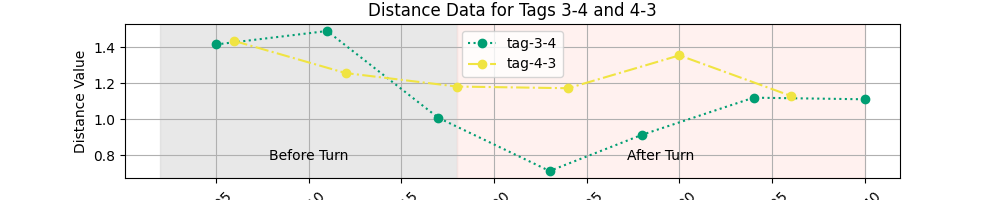
\includegraphics[width=\linewidth]{graphics/exp/exp4_2_gyro_split_distance_3_4.png}
	\caption{Experiment 3, split distance measurement between Tag-3 and Tag-4 over time.}
	\label{f:exp4_graphs_dist_split_3_4}
\end{figure}

\subsection{Colclusion}
\label{s:exp_3_conclusion}
The orientational read of the gyroscope produces puzzeling rezluts.
Many values are zero for most of the time, but not consistently.
This does not make any sense, since the orientational read does not reset after it has been read, rather it updates continously.
For a measurement to reutrn to zero after a wrong value, it would need to make the exact same mistake again in reverse.
This seems highly unlikely, escpecialy for it to happen four times in one experiment.
Additionaly, the one orientation that should change, because it was physically turned, remains at zero before and after the turn.
The most plausible explenation for this behaviour is, that their is an error in the implementation of the gyrosscope module when performing read.
Errors that could lead to such behaviour would be, if the orientational values could reset at runtime or if the wrong values are returned when queried.


The angular velocity read on the other hand produces usefull results.
The turn of tag 2 is very visible, while the other tags remain unaffected.
The angular velocity aaround the X axis for Tag-2 reaches a maximal value of 6322 during this reading.
While this might seem like a high value, it would mean that the turning of the tag, if performed at maximum speed constantly, would have taken 0.05s.
Taking into account that this was a maximum speed and that a human can turn something quite fast, this seems like a reasonable result.\\
Axis Y and Z show a rotational high velocity as well, even it is still smaller by a factor of ten than the rotation around the X-Axis.
Since the sensor was attached on the cardboard by zip ties, it would have had some room to move during the turn.
Additionaly since the turn was performed by hand, it is reasonable to assume, that it was not performed perfectly around the X-axis.
These to effects in combination could account for the high angular velocities around the unaffected Axis.
These results show, that the angular read can be used to detect rotational movement on the Tag. \\
In addition we get an estimate for the biases of the MPU6050.
It appears that the sensor outputs an angular velocity between $0\frac{\degreem}{s}$ and 50 $0\frac{\degreem}{s}$.
While this does not explain the result for the orientational read by itself, it may inform those readings.

During the orientational experiment, the Tag was turned around the Z-Axis, with an atempt beeing made to keep the MPU6050 sensor in the center.
This moved the antenna of the DWM3000 board closer to the tag 1 and further away from Tag-3 and Tag-4.
This behaviour was captured by the distance measurements.
While the distance values are still not correct, even the differences, it caputes something that actually happened in during the experiment.\\
Since the results of the oritentational read were already known during the angular velocity read experiment, a descision was made to test, if a better turn could prevent the distance read.
Instead of the Z-axis, the X-Axis was chosen for the turn, since it corresponds to the antenna position of the DWM3000 baord.
Additionaly the turn was centered around the DWM3000 shield instead of the MPU6050.
This results in the turn not beeing visible in the distance reads from the experiment.\\
It is unclear why the distance measurements between Tag-3 and Tag-4 were inconsisten, when originating with Tag-3. 
Both tags were not part of the experiment.
If a repeated multipath-effect would appear, it should affect both mesurments euqaly, since both participate in DS-TWR.
Tag-4 served as the connection to the Phone in this experiment.
It is possible, that a poor interaction between the BLE and UWB systems happened.
It would be surprising, that these errors only appeared, when Tag-4 was participating, but not initiating the ranging session.


\section{Experiment 4: Distance}
\label{ss:exp_4}
The same 80 cm by 50 cm rectangle setup was used as in previous experiments.
The tags were turned on sequentilay, giving them enough time to build the network.
The phone was connected to one tag.
The max distance parameter was set to 20 centimeter.
After 20 minutes, Tag-1 was moved parallel to the shorter rectangle line about 20 cm towards Tag-2 on the next corner.
Figure \ref{f:exp4_schematic} shows a schemativ view of the experiment.
The system was then left resting for another 30 minutes.
The goal of experiment 4 was to test the detection of unwanted movement.


\begin{figure}[ht!]
	\centering
	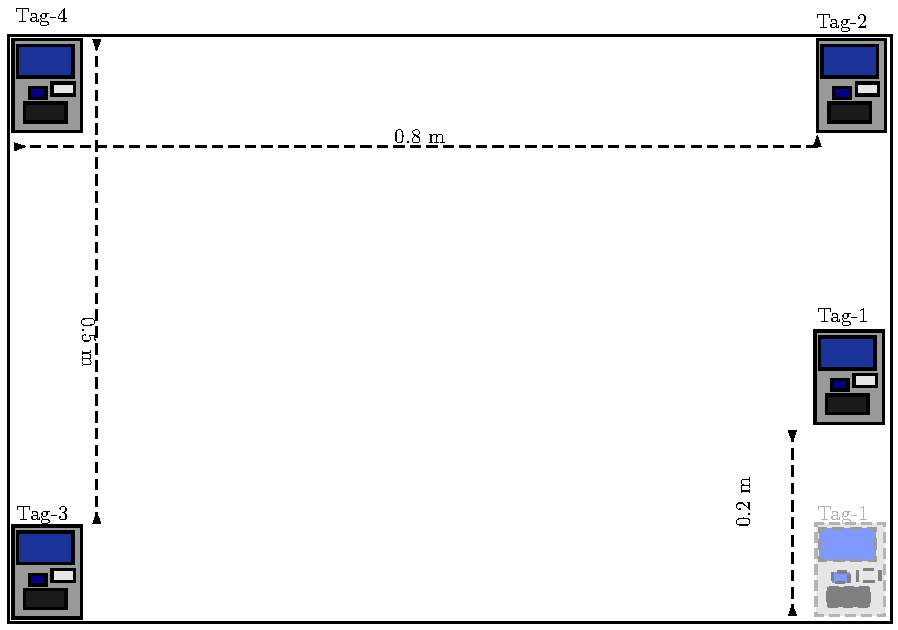
\includegraphics[width=300px]{graphics/schematics/experiment_4.pdf}
	\caption{Schema of the setup of experiment 4.}
	\label{f:exp4_schematic}
\end{figure}

\subsection{Results}
\label{ss:exp_4_result}

Experiment four was intended to test the distance measurement capabilities of the setup.
Temperature and humidity and gyro behave as they do in experiment 1 \ref{ss:exp_1_result}.
For the gyroscopic data, the orientational read was used.
It presents the same issues as in experiment 1 and 3.
Humdity, Temperature adn Gyroscope will not be discussed further for tis experiment.

\begin{figure}[ht!]
	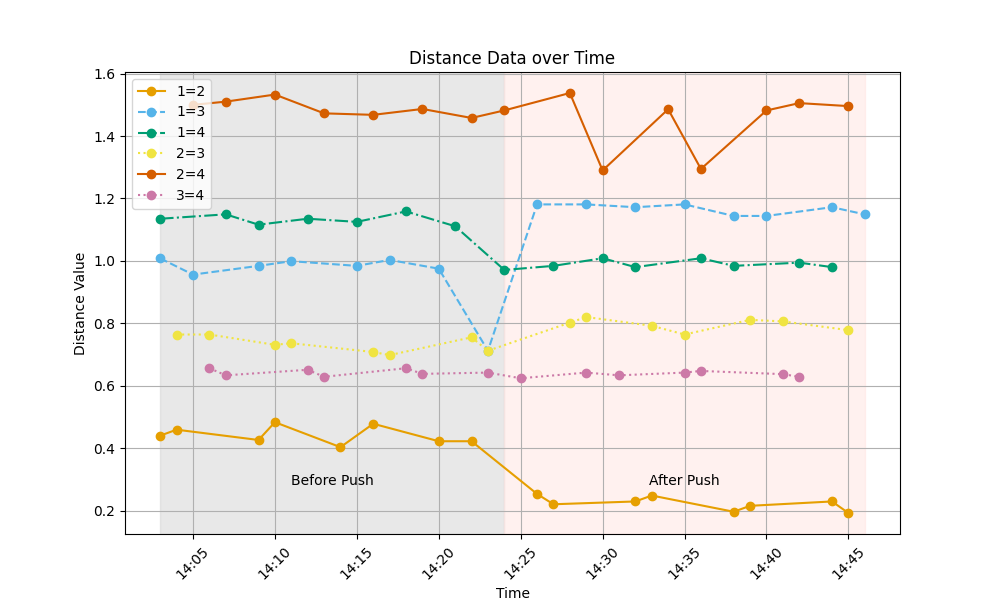
\includegraphics[width=\linewidth]{graphics/exp/exp5_dist_data_plot_2_combined.png}
	\caption{Experiment 4, pairs of distance over time.}
	\label{f:exp3_graphs_dist}
\end{figure}


As with previous distance measurements, the pairs of distances moved together.
Figure \ref{f:exp5_graphs_dist} shows the measured distance pairs of the 4 tags over time.
At 14.24 Tag-1 was moved by 0.23 meters toward Tag-2.
The time before the push has a gray background, while the time after the push has red one.
The measured distances from Tag-1 to Tag-3 increases, while the distance to Tags-2 and Tag-4 dicreases.
This represent what is happening in reality, since Tag-1 is now closer to Tag-2 and Tag-4 and further away from Tag-3 as before.

\begin{figure}[ht!]
	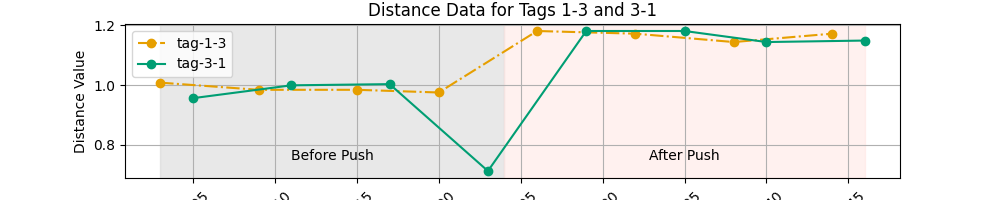
\includegraphics[width=\linewidth]{graphics/exp/exp5_dist_data_plot_2_split_1_3.png}
	\caption{Experiment 4, distance between Tag-1 and Tag-3}
	\label{f:exp3_graphs_dist_split_1_3}
\end{figure}


Table \ref{tab:exp4_mean_distances} shows the mean values of distance pairs before and after the move.
The variances for all values, are low, confirming the choice to combine pairs during evaluation.
As in experiment 1 and 3, the reported distances do not correspond to the what is phisically happending.
The difference in mean distance 1=2 before and after the push is 0.209m.
This is close to the 0.23m that Tag-1 was acutally moved to Tag-2.
The measurements show Tag-4 0.144m closer to Tag-1 after the push.
The effect on tag 4 should be notissable but not as large as it is.
Since the tag moves lateraly towards tag 4, the difference should only be 0.03 meters.
The difference in measured distance between Tag-1 and Tag-3 is 0.213 meters.
Figure \ref{f:exp3_graphs_dist_split_1_3} shows the distance measurements between Tag-1 and Tag-3.
Measurement 1-3 and 3-1 move together as a pair, ecepct for the fourth measurement of distance 3-1.
This also shows the higher variance of pair 1=3.
If the outlier value is ignored, the distance difference between the means beofre and after the oush becomes 0.179 meters. 
This is still too large for the difference a latteral move, it should only be a 0.100 m difference.
Their is also a small increase in the distance between tags 2 and 3, but which starts before tag 1 was moved.


\begin{table}[ht]
\centering
\caption{Statistics of the combined distance measurements between tags before and after the push for experiment 4}
\begin{minipage}{0.45\textwidth}
\centering
\begin{tabular}{|c|c c c|}
\hline
		& \textbf{Tag-2} & \textbf{Tag-3} & \textbf{Tag-4} \\
\hline
\textbf{Tag-1}    & 0.442 & 0.953 & 1.133 \\
\textbf{Tag-2}   &  & 0.734 & 1.490 \\
\textbf{Tag-3}   &  &  & 0.654 \\
\hline
\end{tabular}
\caption*{Mean before move}
\end{minipage}
\hfill
\begin{minipage}{0.45\textwidth}
\centering
\begin{tabular}{|c|c c c|}
\hline
		& \textbf{Tag-2} & \textbf{Tag-3} & \textbf{Tag-4} \\
\hline
\textbf{Tag-1}    & 0.223 & 1.166 & 0.989 \\
\textbf{Tag-2}   &  & 0.796 & 1.447 \\
\textbf{Tag-3}   &  &  & 0.635 \\
\hline
\end{tabular}
\caption*{Mean afer move}
\end{minipage}
\hfill
\begin{minipage}{0.45\textwidth}
\centering
\begin{tabular}{|c|c c c|}
\hline
		& \textbf{Tag-2} & \textbf{Tag-3} & \textbf{Tag-4} \\
\hline
\textbf{Tag-1}    & 0.000 & 0.010 & 0.000 \\
\textbf{Tag-2}   &  & 0.001 & 0.001 \\
\textbf{Tag-3}   &  &  & 0.000 \\
\hline
\end{tabular}
\caption*{Variance before move}
\end{minipage}
\hfill
\begin{minipage}{0.45\textwidth}
\centering
\begin{tabular}{|c|c c c|}
\hline
		& \textbf{Tag-2} & \textbf{Tag-3} & \textbf{Tag-4} \\
\hline
\textbf{Tag-1}    & 0.000 & 0.000 & 0.000 \\
\textbf{Tag-2}   &  & 0.000 & 0.010 \\
\textbf{Tag-3}   &  &  & 0.000 \\
\hline
\end{tabular}
\caption*{Variance afer move}
\end{minipage}
\label{tab:exp4_mean_distances}
\end{table}

\subsection{Conclusion}
\label{s:exp_4_conclusion}
As was shown in Experiment 1, the distances do not match with the phsiscal distances.
However, the differences in distance materialize correctly.
The correct distances increase and dicrease to match the physical reality.
The most probable reason for the incorrect distances is the simplified calibration.
The difference between the correct and measured distances never exeeds 0.4m, which is the assumed error by Qorvo, when using incorrect calibration.\\
The difference in distance is even closer, onyl beeing off by 0.1m at most.
For now this error is still too large to be used unmodified in real world applications.


\section{Experiment 5: Real World experiment}
\label{s:exp_5_real_world}
Experiment 5 was designed to check, how the setup would do in a real world applicaion.
For this, all tags were put in a rucksack and taken on a journey.
To protect the electronics from damage, each tag was put in a transparent cylindrical plastic bucket with radiu 012m and a hight of 0.14m and no lid.
The buckets in the rucksack were stacked so there were two next to each other at the bottom and two on top.\\
First, the rucksack was taken by foot from Binzmmühlstrasse 14 by foot to the Zurich Oerlokon train staiton.
From their the journey continued via train to Zurich Main Station.
After a short walk in Zurich Main Station, the journey continued via train to Lenzburg, were the jouney ended at the Lenzburg train station. \\
During the whole journey, the backpack was on the back of the person conductung the experiment and was nether put on the floor.
This was done to protect the electronics from potential accidents by careless travelers during rush-hour.

\subsection{Results}
\label{s:exp5_real_worl_results}
The walk by foot began at 17.43 and ended 17:51 when the S6 train to the main station was entered.
The S6 arrived at the main station at 18:01.
From their the track had to be changed and 18.08 the train to Lenzburg was entered.
The train drove for 24 minutes, until the experiment ended 18:32 at the Lenzburg trainstation.\\
The following section will contain Figures for this journey.
The figure all use the same color scheme to describe the journey.
The first part by foot will have a gray background.
The first trinride in the S6 will have a red background.
The time in Zurich Main Station is blue and the final trainride to Lenzburg green.

\begin{figure}[ht!]
	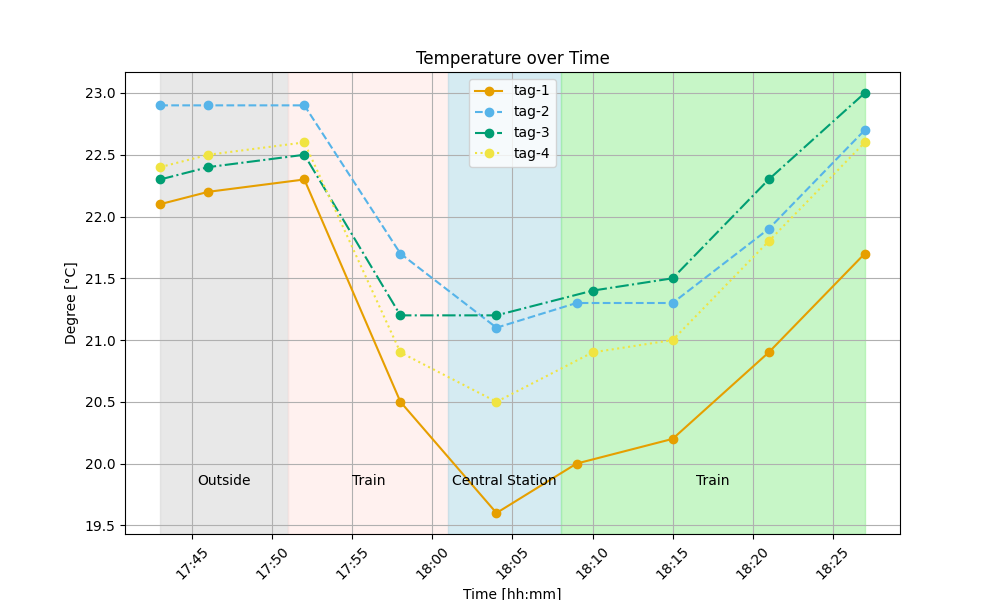
\includegraphics[width=\linewidth]{graphics/exp/exp6_temp_plot_2.png}
	\caption{Temperature over time during experiment 5.}
	\label{f:ex5_train_temp}
\end{figure}

Figure \ref{f:ex5_train_temp} shows the measured temperatures during experiment 5.
All four tags start with a high temperature between 22\degree and 23\degree .
This remains true until the train is reached, were the temperatures start drop during the second measurement in the train to by a bit over one degree to a range of 20.5\degree to 21.7\degree .
During the one measurement in the main station, most tags have their lowset values during the whole experiment, Tag-1 with 19.6\degree , Tag-2 with 21.1\degree and Tag-4 with 20.5\degree .
The only tag without a significant drop during the main station is Tag-3, which records the same temperature of 21.2\degree as in the previous train.
During the second train ride, all tags report a stadely increasing temperature. \\
Tag-2 starts with the a temperature that is 0.5\degree higher than the other tags, who all start with very close values.
Tag-1, Tag-3 and Tag-4 stay close until the first train ride.
From there on Tag-1 drops to lower temperature measurements that are 1\degree lower than the lowest measurement of the rest, Tag-4, and stays there until the rest of the experiment.
Tag-2 and Tag-3 report similar values during the Main Station and keep having similar values until the end.
Tag-4 reports values that are close to Tag-2 and Tag-3, but alwys below it. This becomes specialy pronounced at the main station, where Tag-4 measures 20.5\degree , 0.6 \degree lower than Tag-2 and 0.7 \degree lower than Tag-3.




\begin{figure}[ht!]
	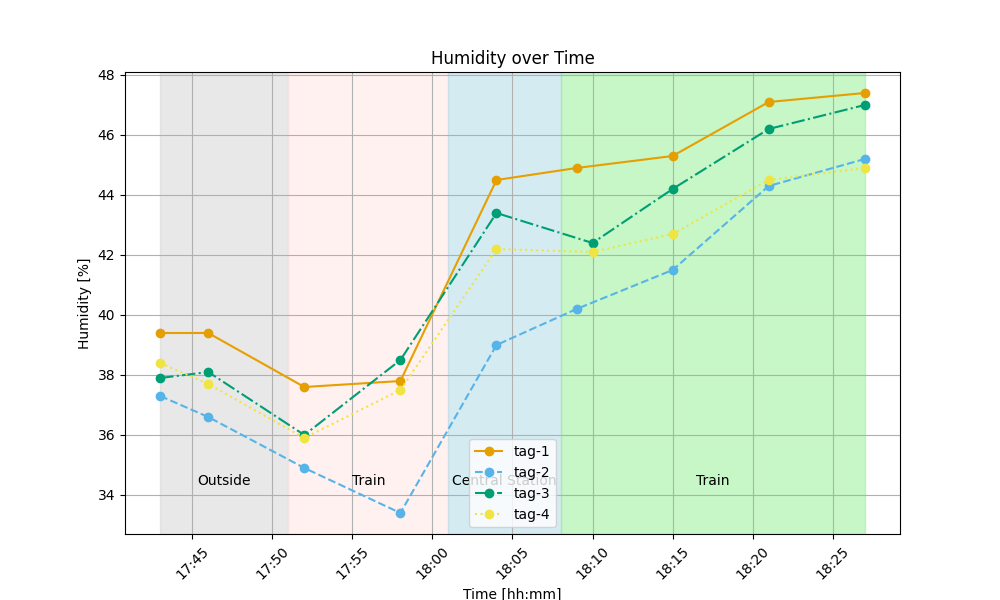
\includegraphics[width=\linewidth]{graphics/exp/exp6_hum_plot_2.png}
	\caption{Humidity over time during experiment 5.}
	\label{f:ex5_train_hum}
\end{figure}